\section{Figures}
\label{sec:figures}

%\subsection{Figures to section \ref{sec:data}}


\begin{figure}[h]
\centering
%l b r t
\caption{Aggregate number of job openings, from survey, 2001-2012}
\includegraphics[trim = 0mm 0mm 0mm 0mm, clip, scale=.75]{\datadir Data/Not_Server/SCB/figures/fig_survey_private_vacancies.pdf}
\begin{flushleft}
\footnotesize{\emph{Notes:} The figure shows the aggregate number of job openings in the \emph{Job Vacancy Survey} on quarterly frequency. Sample is restricted to private sector.} \\ 
\footnotesize{\emph{Sources:} Statistics Sweden.} 
\label{fig:survey_openings_timeserie}
\end{flushleft}
\vspace{3mm}
\centering
%l b r t
\caption{Distribution of vacancies at the plant-level}
\includegraphics[trim = 0mm 3mm 0mm 0mm, clip, scale=.75]{\datadir Data/Server/figures/plot_survey_openings_hist.pdf}
\begin{flushleft}
%\footnotesize{\emph{Notes:} Mean is 2.2 openings, median is 0, 75p is 1 and 90 is 4.} \\
\footnotesize{\emph{Notes:} The figure shows the distribution of job openings in the \emph{Job Vacancy Survey}.} \\ 
\footnotesize{\emph{Sources:} Statistics Sweden.}
\label{fig:survey_openings_hist}
\end{flushleft}
\end{figure}

%\begin{figure}[t]
%\centering
%%l b r t
%\caption{Aggregate number of job vacancies in Sweden, from Public Employment Service, 2002-2012}
%\includegraphics[trim = 0mm 0mm 0mm 0mm, clip, scale=.75]{\datadir Data/Server/figures/fig_PES_vacancies_timeserie_quarterly.pdf}
%\begin{flushleft}
%\footnotesize{\emph{Notes:} The figure shows the aggregate number of job openings registered at the Public Employment Service on quarterly frequency.} \\ 
%%and Public Employment Service, respectively. The sample of firms is restricted to those sampled in the \emph{Job Vacancy Survey}.} \\
%\footnotesize{\emph{Sources:}  Swedish Public Employment Service.} 
%\end{flushleft}
%\label{fig:PES_openings_timeserie}
%\vspace{2mm}
%\centering
%%l b r t
%\caption{Distribution of vacancies at the firm-level}
%\includegraphics[trim = 0mm 2mm 0mm 0mm, clip, scale=.75]{\datadir Data/Server/figures/plot_PES_openings_hist.pdf}
%\begin{flushleft}
%\footnotesize{\emph{Notes:} The figure shows distribution of vacancies registered at the Public Employment Service. } \\
%%The sample are the \emph{firms} surveyed in the \emph{Job Vacancy Survey}. 
%\footnotesize{\emph{Sources:} The Swedish Public Employment Service.}
%\end{flushleft}
%\label{fig:PES_openings_hist}
%\end{figure}

	
\begin{figure}[t]
\centering
%l b r t
\caption{Aggregated survey hires, private sector, 2001-2012}
\label{fig:hires_survey_timeserie}
\includegraphics[trim = 0mm 0mm 0mm 0mm, clip, scale=0.75]{\datadir Data/Not_Server/SCB/figures/fig_survey_private_hires.pdf}
%{../../Data/Server/figures/fig_survey_hires_timeserie.pdf}
\begin{flushleft}
\footnotesize{\emph{Notes:} The figure shows the number of hires \emph{Short-Term Employment Statistics}. Only private sector is included due to databreak in time-series for public sector.} \\
%\footnotesize{\emph{Sources:} Institute for Evaluation of Labour Market and Education Policy and the \emph{Short-Term Employment Statistics} from Statistics Sweden.}
\footnotesize{\emph{Sources:} Statistics Sweden.}
\end{flushleft}
\vspace{2mm}
\centering
%l b r t
\caption{Distribution of survey hires at the plant-level}
\label{fig:hires_survey_hist}
\includegraphics[trim = 0mm 0mm 0mm 0mm, clip, scale=0.75]{\datadir Data/Server/figures/plot_survey_hires_hist.pdf}
\begin{flushleft}
\footnotesize{\emph{Notes:} The figure shows the histogram of hires at plant level from the \emph{Short-Term Employment Statistics} } \\
\footnotesize{\emph{Sources:} Statistics Sweden.}
\end{flushleft}
\end{figure}

\begin{figure}[t]
\centering
%l b r t
\caption{Aggregated tax hires, 2002-2012}
\label{fig:hires_tax_timeserie}
\includegraphics[trim = 0mm 0mm 0mm 0mm, clip, scale=.75]{\datadir Data/Server/figures/fig_tax_hires_timeserie_quarterly.pdf}
\begin{flushleft}
\footnotesize{\emph{Notes:} The figure shows the aggregate number of hires derived from the tax data. Method is described in \ref{sec:data}.} \\
\footnotesize{\emph{Sources:} Institute for Evaluation of Labour Market and Education Policy.}
\end{flushleft}

\vspace{5mm}
\centering
%l b r t
\caption{Distribution of hires at the plant-level}
\label{fig:hires_tax_hist}
\includegraphics[trim = 0mm 5mm 0mm 0mm, clip, scale=.75]{\datadir Data/Server/figures/plot_tax_hires_hist.pdf}
\begin{flushleft}
\footnotesize{\emph{Notes:} The figure shows the distribution of hires at the plant level. The sample of plants is restricted to those sampled in the \emph{Short-Term Employment Statistics}.} \\
\footnotesize{\emph{Sources:} Institute for Evaluation of Labour Market and Education Policy and Statistics Sweden.}
\end{flushleft}
\end{figure}

\begin{figure}[t]
\centering
%l b r t
\caption{Monthly hires in Sweden, tax and survey hires, 2002-2012}
\label{fig:hires_tax_survey_timeserie}
\includegraphics[trim = 0mm 0mm 0mm 0mm, clip, scale=.75]{\datadir Data/Server/figures/fig_survey_tax_hires_timeserie.pdf}
\begin{flushleft}
\footnotesize{\emph{Notes:} The figure shows the number of hires derived from the tax and survey data. Sample of plants is as in the \emph{Short-Term Employment Statistics}.} \\
\footnotesize{\emph{Sources:} Institute for Evaluation of Labour Market and Education Policy and Statistics Sweden.}
\end{flushleft}
\end{figure}


%% Relationship between vacancies and hires on plant level %%
%\FloatBarrier
%\subsection{Figures to section \ref{sec:basic_rel}}


\begin{figure}[t]

\centering
%l b r t
\caption{Plant-level relationship between vacancies and tax hires}
\includegraphics[trim = 0mm 5mm 0mm 0mm, clip, scale=.75]{\datadir Data/Server/figures/plot_medio_survey_v_tax_hires_integer.pdf}
\flushleft
\footnotesize{\emph{Notes:} The figure shows the average number of hires (y-axis) for each number of vacancies in the previous month (x-axis). Period is 2001-2012. Hires are measured via tax data. The solid line denotes the 45-degree line.} \\
\footnotesize{\emph{Source:} Own calculation on data from Statistics Sweden and IFAU.}
\label{fig:crossplot_using_tax_hires}

\vspace{2mm}

\centering
%l b r t
\caption{Plant-level relationship between vacancies and survey hires}
\includegraphics[trim = 0mm 5mm 0mm 0mm, clip, scale=.75]{\datadir Data/Server/figures/plot_medio_survey_v_survey_hires_integer.pdf}
\flushleft
\footnotesize{\emph{Notes:} The figure shows the average number of hires (y-axis) for each number of vacancies in the previous month (x-axis). Period is 2001-2012. Hires are measured via survey data. The solid line denotes the 45-degree line.} \\
\footnotesize{\emph{Source:} Own calculation on data from Statistics Sweden.}
\label{fig:crossplot_using_survey_hires}

\end{figure}

\begin{figure}[t]
\centering
%l b r t
\caption{Share of hires without vacancies in the preceding month, 2002-2012}
\includegraphics[trim = 0mm 0mm 0mm 0mm, clip, scale=.75]{\datadir Data/Server/figures/plot_share_hire_without_vacancies.pdf}
\flushleft
\footnotesize{\emph{Notes:} This figure shows the share of hires, that are made without a vacancy present in the previous month in the given plant. An average is computed for each year. The figure is done using both hires from tax and survey data.} \\
\footnotesize{\emph{Source:} Own calculations on data from Statistics Sweden and IFAU.}
\label{fig:share_without}
\end{figure}

\begin{figure}[t]
\centering
%l b r t
\caption{Duration of vacancies at the Public Employment Service, 2001-2012}
\includegraphics[trim = 0mm 0mm 0mm 0mm, clip, scale=.75]{\datadir Data/Server/figures/plot_PES_duration.pdf}
\flushleft
\footnotesize{\emph{Notes:} The figure shows the histogram of the interval between start and end date of all vacancies registered at the Public Employment Service during the period 2001-2013.} \\
\footnotesize{\emph{Source:} The Swedish Public Employment Service.}
\label{fig:PES_duration}
\end{figure}

%% Figures to time aggregation %%%
%\FloatBarrier
%\subsection{Figures to section \ref{sec:time_agg}}

\begin{figure}[t]
\centering
%l b r t
\caption{Timing of vacancy and hires observations in data}
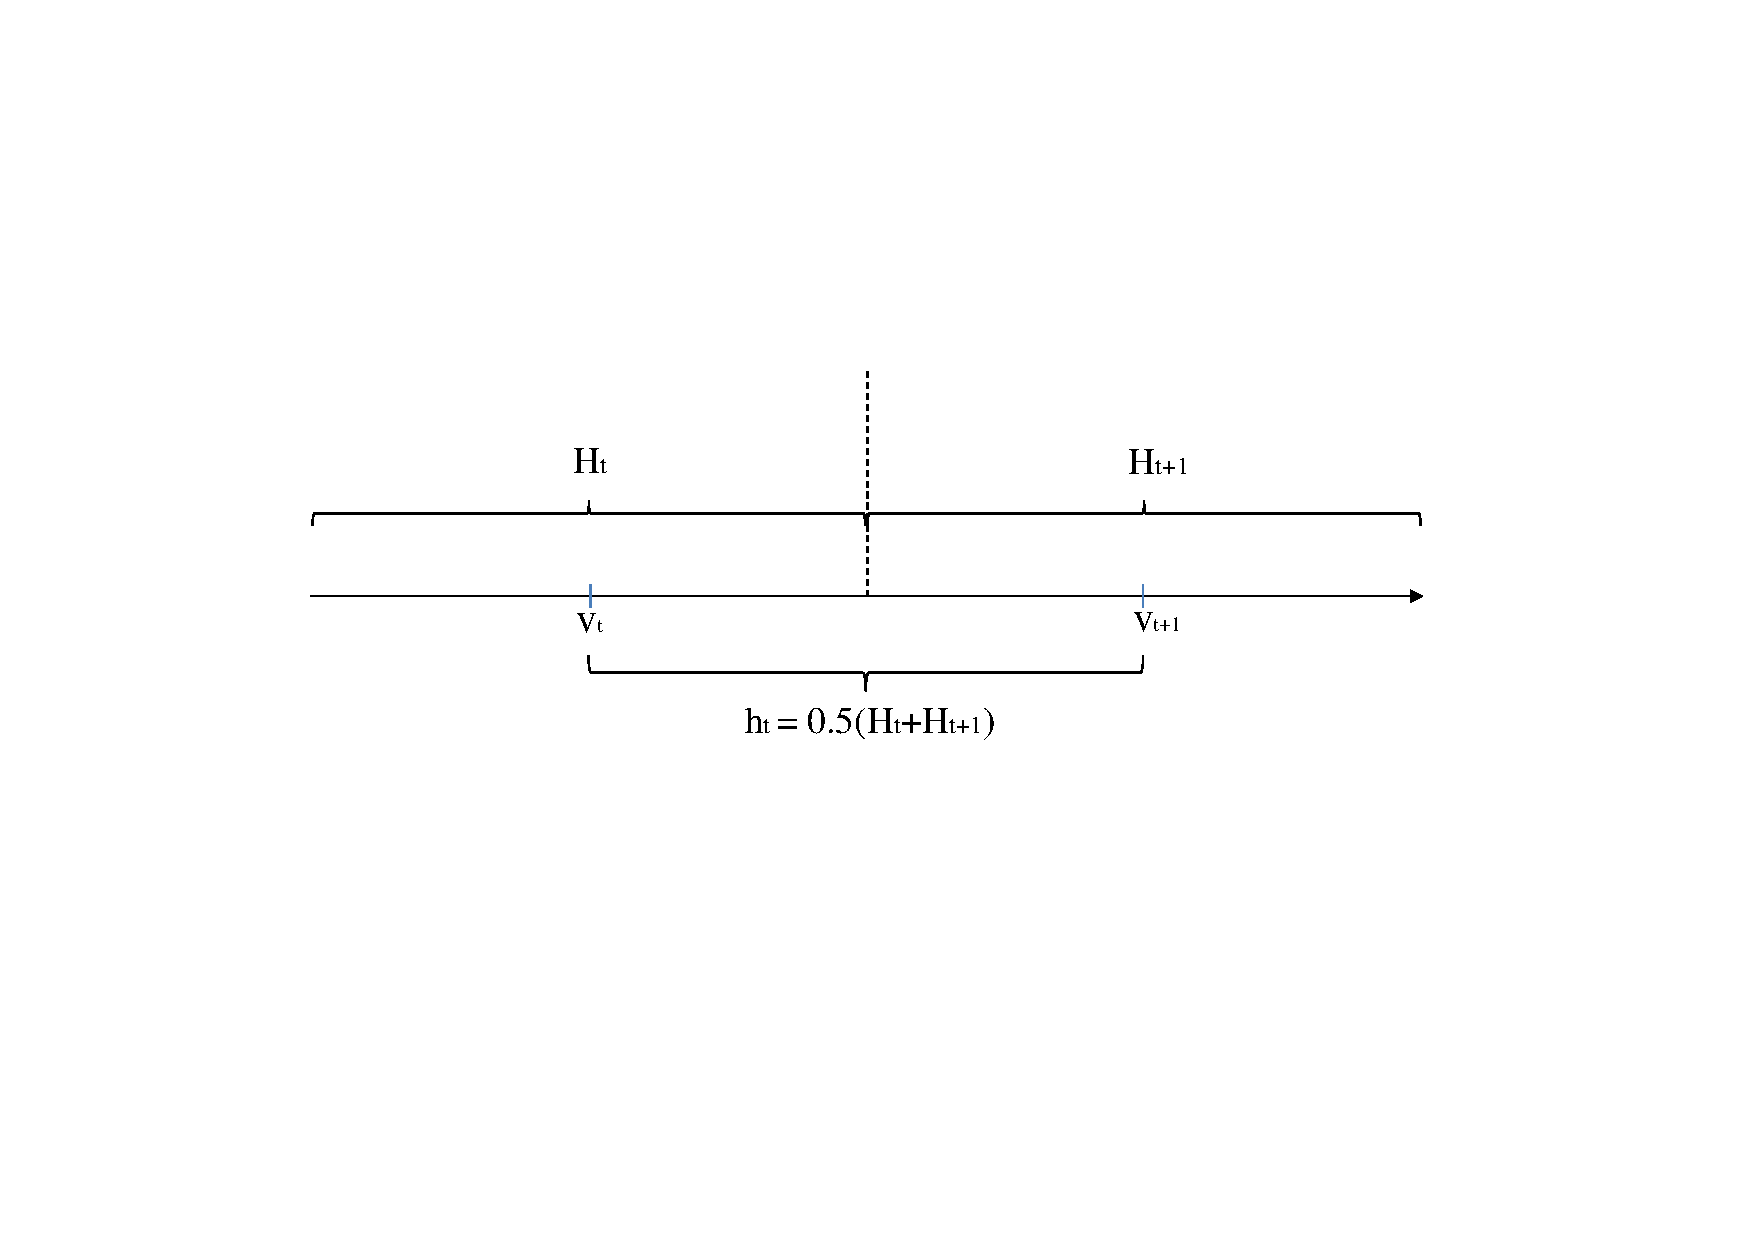
\includegraphics[trim = 20mm 80mm 40mm 60mm, clip, width=\textwidth]{\datadir timagg/timing_illu}
\flushleft
\footnotesize{}
\label{fig:timing_illustration}
\end{figure}

%\begin{figure}[t]
%\centering
%l b r t
%\caption{Aggregated survey vacancies, private sector, 2001-2012}
%\label{fig:aggregate_survey_vacancies}
%\includegraphics[trim = 0mm 0mm 0mm 0mm, clip, scale=.96]{../../Data/Not_Server/SCB/figures/fig_survey_vacancies_timeseries_quarterly_scb.pdf}
%\begin{flushleft}
%\footnotesize{\emph{Notes:} The figure shows the aggregated number of vacancies in the private sector as published in the \textit{Swedish Job Vacancy Survey}.} \\
%\footnotesize{\emph{Sources:} Statistics Sweden.}
%\end{flushleft}
%\vspace{5mm}
%\centering
%l b r t
%\caption{Aggregated survey hires, private sector, 2001-2012}
%\label{fig:aggregate_survey_hires}
%\includegraphics[trim = 0mm 0mm 0mm 0mm, clip, scale=.96]{../../Data/Not_Server/SCB/figures/fig_survey_hires_timeseries_quarterly_scb.pdf}
%\begin{flushleft}
%\footnotesize{\emph{Notes:} The figure shows the aggregated number of hires in the private sector as published in \emph{Short-Term Employment Statistics}.} \\
%\footnotesize{\emph{Sources:} Statistics Sweden.}
%\end{flushleft}
%\end{figure}

\begin{figure}[t]
\centering
%l b r t
\caption{Daily Job-Filling Rates, private sector, 2001-2016}
\label{fig:aggregate_filling_rates}
\includegraphics[trim = 0mm 0mm 0mm 0mm, clip, scale=.75]{\datadir timagg/output/fig_filling_rate_total}
\begin{flushleft}
\footnotesize{\emph{Sources:}  Own calculations on data from Statistics Sweden.}
\end{flushleft}
\vspace{5mm}

\centering
%l b r t
\caption{Monthly Flow Rates of New Vacancies, private sector, 2001-2016}
\label{fig:aggregate_creation_rates}
\includegraphics[trim = 0mm 0mm 0mm 0mm, clip, scale=.75]{\datadir timagg/output/fig_vacan_rate_total.pdf}
\begin{flushleft}
\footnotesize{\emph{Sources:} Own calculations on data from Statistics Sweden.}
\end{flushleft}
\end{figure}

\begin{figure}[t]
\centering
%l b r t
\caption{Share of hires without vacancies in the preceding month, 2001-2012. \newline Corrected for time-aggregation}
\includegraphics[trim = 0mm 0mm 0mm 0mm, clip, scale=.80]{\datadir Data/Server/figures/plot_share_hire_without_vacancies_timeagg.pdf}
\flushleft
\footnotesize{\emph{Note:} Figure depicts share of $h_{t,corrected}$ with $v_{t-1,ultimo}$ being above one, where $v_{t-1,ultimo}$} \\
\footnotesize{ has been rounded to nearest integer. } \\
\footnotesize{\emph{Source:} Own calculation on data from Statistics Sweden.}
\label{fig:share_without_timeagg}
\end{figure}

\FloatBarrier

%% Figures to aggregate implications %%%
%\FloatBarrier
%\subsection{Figures to section \ref{sec:agg_implications}}

%% Job-openings using the traditional and alternative measure
\begin{figure}[h]
\centering
%l b r t
\caption{Job-openings, traditional and alternative measure}
\includegraphics[trim = 0mm 10mm 0mm 0mm, clip, width=0.9\textwidth]{\datadir Data/Not_Server/Matching_estimation/figures/fig_vac_measure_activeplants.pdf}
\begin{flushleft}
%\footnotesize{\emph{Notes:} The figure shows job-openings on the labor market measured via the traditional and alternative measure, respectively. The traditional measure uses vacancy as measure of job-openings. The alternative uses the sum of plants with any vacancies weighted by number of employees. Data is seasonally adjusted. Shaded area are the years with declining economic activity (2008-09)} \\
%\footnotesize{\emph{Source:} Own calculation on data from Statistics Sweden.}
\end{flushleft}
\label{fig:openings_std_and_alt}
\vspace{0mm}
\centering
%l b r t
%\caption{Job-openings, traditional and alternative measure}
\includegraphics[trim = 0mm 10mm 0mm 0mm, clip, width=0.9\textwidth]{\datadir Data/Not_Server/Matching_estimation/figures/fig_vac_measure_activeplants_empw.pdf}
\begin{flushleft}
\footnotesize{\emph{Notes:} The figures show job-openings on the labor market measured via the traditional and the two alternative measures, respectively. In the upper panel the alternative measure is the number of plants with a positive number of vacancies. In the lower panel it is the number of plants with a positive number of vacancies, weighted by employment shares. Data is seasonally adjusted. Shaded area are the years with declining economic activity (2008-09)} \\
\footnotesize{\emph{Source:} Own calculation on data from Statistics Sweden.}
\end{flushleft}
\end{figure}


%% Labor market tightness using the traditional and alternative measure
\begin{figure}[h]
\centering
%l b r t
\caption{Labor market tightness, traditional and alternative job-opening measure}
\includegraphics[trim = 0mm 10mm 0mm 0mm, clip, width=0.9\textwidth]{\datadir Data/Not_Server/Matching_estimation/figures/vu_unweighted.pdf}
\flushleft
%\footnotesize{\emph{Notes:} The figure shows labor market tightness defined as the stock of job-openings divided by the stock of unemployed. The traditional measure uses vacancy as measure of job-openings. The alternative uses the sum of plants with any vacancies weighted by number of employees. Data is seasonally adjusted. Shaded area are the years with declining economic activity (2008-09).} \\
%\footnotesize{\emph{Source:} Own calculation on data from Statistics Sweden.}
\label{fig:tightness}
\vspace{0mm}
\centering
\includegraphics[trim = 0mm 10mm 0mm 0mm, clip, width=0.9\textwidth]{\datadir Data/Not_Server/Matching_estimation/figures/vu_weighted.pdf}
\flushleft
\footnotesize{\emph{Notes:} The figure shows labor market tightness defined as the stock of job-openings divided by the stock of unemployed. The traditional measure uses vacancy as measure of job-openings. In the upper panel the alternative measure is the number of plants with a positive number of vacancies. In the lower panel it is the number of plants with a positive number of vacancies, weighted by employment shares.  Shaded area are the years with declining economic activity (2008-09).} \\
\footnotesize{\emph{Source:} Own calculation on data from Statistics Sweden.}
\label{fig:tightness}
\end{figure}


%% Share of plants with zero vacancies
%\begin{figure}[h]
%\centering
%%l b r t
%\caption{Share of plants with zero reported vacancies}
%\includegraphics[trim = 0mm 0mm 0mm 0mm, clip, width=\textwidth]{../../Data/Server/figures/share_with_zero_vacancies.pdf}
%\flushleft
%%\footnotesize{\emph{Notes:} } \\
%%\footnotesize{\emph{Source:} Own calculation on data from Statistics Sweden.}
%\label{fig:plants_zero_vacan}
%\end{figure}

%% Vacancies across plant size
\begin{figure}[h]
\centering
%l b r t
\caption{Vacancies across the size distribution, private sector}
\includegraphics[trim = 0mm 0mm 0mm 0mm, clip, width=0.9\textwidth]{\datadir Data/Server/figures/plot_vacancies_across_size.pdf}
\flushleft
\footnotesize{\emph{Notes:} The figure shows the development in the average number of job-openings, as measured in the survey, across the plant-size. When adding up the number of vacancies sample weights have been applied. Public sector has been excluded due to data break in 2006.} \\
\footnotesize{\emph{Source:} Own calculation on data from Statistics Sweden.}
\label{fig:vacancies_across_size}
\end{figure}


%\begin{figure}[h]
%\centering
%%l b r t
%\caption{Average job-openings across the size distribution}
%\includegraphics[trim = 0mm 0mm 0mm 0mm, clip, width=\textwidth]{../../Data/Server/figures/plot_avg_survey_vacancies_per_year.pdf}
%\flushleft
%\footnotesize{\emph{Notes:} The figure shows the development in the average number of job-openings, as measured in the survey, across the plant-size percentiles . \emph{E.g.} 0-20 \% shows the development in the average number of job-openings in among the 20 \% plants with the fewest employees.} \\
%\footnotesize{\emph{Source:} Own calculation on data from Statistics Sweden.}
%\label{fig:estimated_jfr}
%\end{figure}

\begin{figure}[h]
\centering
%l b r t
\caption{Actual and predicted job-finding rate, traditional and alternative job-opening measure}
\includegraphics[trim = 0mm 0mm 0mm 0mm, clip, width=0.9\textwidth]{\datadir Data/Not_Server/Matching_estimation/figures/jfr_traditional_and_alternative_measure_weighted.pdf}
\flushleft
\footnotesize{\emph{Notes:} Figure shows the actual and predicted job-finding rate estimated via the traditional and alternative measure of job-openings as input into the estimated matching function (Table \ref{tab:matchning_nsa}). The matching function is estimated on data up to the beginning of 2008. Shaded area are the years with declining economic activity (2008-09).} \\
\footnotesize{\emph{Source:} Own calculation on data from Statistics Sweden.}
\label{fig:estimated_jfr}
\end{figure}

\begin{figure}[h]
\centering
%l b r t
\caption{Beveridge curves}
%\includegraphics[trim = 0mm 0mm 0mm 0mm, clip, width=\textwidth]{../../Data/Not_Server/Matching_estimation/figures/BC_std_v_activeplants_weighted.pdf}
\includegraphics[trim = 0mm 0mm 0mm 0mm, clip, width=0.9\textwidth]{\datadir Data/Not_Server/Matching_estimation/figures/BC_activeplants_empw_grey.pdf}
\flushleft
\footnotesize{\emph{Notes:} \enquote{Standard} shows the Beveridge curve drawn using the standard vacancy measure for job-openings. \enquote{Alternative} shows the Beveridge curve drawn when using the number of plants with a positive number of vacancies weighted by their share of employment.} \\
\footnotesize{\emph{Source:} Own calculation on data from Statistics Sweden.}
\label{fig:Beveridge}
\end{figure}

%% Kappa measure and predicted finding rates
\begin{figure}[t]
\centering
%l b r t
\caption{Contribution to job-finding probability from distribution of vacancies}
\label{fig:agg_imp:omegatimeseries}
\includegraphics[trim = 0mm 10mm 0mm 0mm, clip, scale=0.75]{\datadir Data/Not_Server/Matching_estimation/figures_kappa/kappa_measure.pdf}
\begin{flushleft}
\footnotesize{\emph{Notes:} The figure shows the time series for $\log \left( \sum_s \kappa(s) \theta(s, t)  \right)$. That is, size specific matching efficiencies weighted with the distribution of plants across the size distribution. Shaded area are the years with declining economic activity (2008-09).} \\ 
\footnotesize{\emph{Sources:} Own calculations on data from Statistics Sweden.} 
\end{flushleft}
\vspace{0mm}
\centering
%l b r t
\caption{Predicted job finding probabilities}
\label{fig:agg_imp:pred_jfp}
\includegraphics[trim = 0mm 10mm 0mm 0mm, clip, scale=0.75]{\datadir Data/Not_Server/Matching_estimation/figures_kappa/jfr_predicted.pdf}
\begin{flushleft}
\footnotesize{\emph{Notes:} The figure reports the predicted job-finding probabilities using (a) the actual distribution of vacancies and (b) letting the distribution of vacancies post 2008 being fixed on the 2008 level. The parameters of the model are estimated on pre-2008 data. Shaded area are the years with declining economic activity (2008-09).} \\ 
\footnotesize{\emph{Sources:} Own calculations on data from Statistics Sweden.}
\end{flushleft}
\end{figure}

%% Actual and predicted job findings probabilities using kappa model
\begin{figure}[t]
\centering
%l b r t
\caption{Actual and predicted job finding probabilities}
\includegraphics[trim = 0mm 8mm 0mm 0mm, clip, scale=.8]{\datadir Data/Not_Server/Matching_estimation/figures_kappa/jfr_actual_predicted.pdf}
\begin{flushleft}
\footnotesize{\emph{Notes:} The figure shows the time series for the actual and predicted job finding probability. The predicted job finding probability is constructed using the model accounting for vacancy distribution. The model is estimated on pre-2008 data. Shaded area are the years with declining economic activity (2008-09).} \\ 
\footnotesize{\emph{Sources:} Own calculations on data from Statistics Sweden.} 
\label{fig:actual_and_predicted_jfp_model_with_distribution}
\end{flushleft}
\end{figure}